\documentclass[]{article}
\usepackage{amsmath}
\usepackage{graphicx}
\graphicspath{ {./images/} }
%opening
\title{Homework 1}
\author{Marwan Kallal}
\setlength{\parindent}{0pt}
\begin{document}

\maketitle


\section{Distance dependence and the path loss exponent.}

\subsection{}
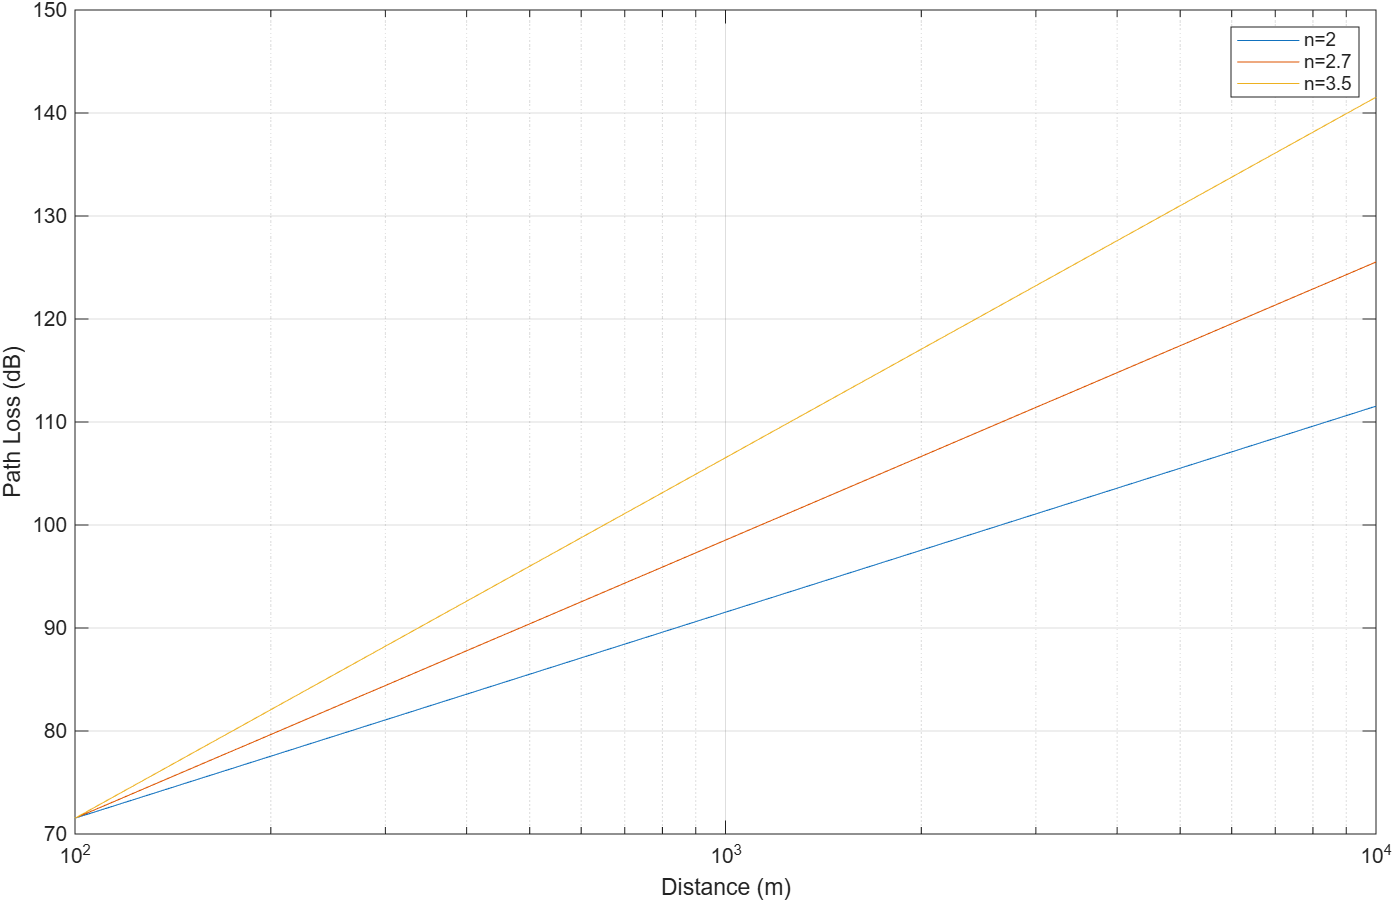
\includegraphics[width=\textwidth]{a_i.png}

\subsection{}
\begin{align*}
	PL_fs|dB &= 32.45 + 20 \log_{10}(f_c(\text{MHz})) + 20 \log_{10}(d(\text{km})) \\
			 &= 32.45 + 20 \log_{10}(900) + 20 \log_{10}(0.1) \\
			 &= 32.45 + 59.08 + (-20) \\
			 &= 71.53 \text{dB}
\end{align*}

\subsection{}
For all $n$: $PL(100m) = 71.53\text{dB}$

For $n=2$: $PL(1000m) = 91.53\text{dB}$, slope $= 20$ dB per decade.

For $n=2.7$: $PL(1000m) = 98.53\text{dB}$, slope $= 27$ dB per decade.

For $n=3.5$: $PL(1000m) = 106.53\text{dB}$, slope $= 35$ dB per decade. \\

The slope in equation 1 is given by $10 n \log_{10}(d/d_0)$, where $d/d_0 = 10$. Importantly, $\log_{10}(10) = 1$.

For $n=2$: slope $= 10 \cdot 2 \log_{10}(10) = 20$ dB per decade.

For $n=2.7$: slope $= 10 \cdot 2.7 \log_{10}(10) = 27$ dB per decade.

For $n=3.5$: slope $= 10 \cdot 3.5 \log_{10}(10) = 35$ dB per decade.

These computed values match the plots.

\subsection{}
For $n=2$, we expect this to be free space.

For $n=2.7$, we expect this to be an urban area.

For $n=3.5$, we expect this to be either an urban area, or an urban area with obstacles in the path.

This change from $n=2$ to $n=3.5$ represents the environment becoming more crowded, with more obstacles in the environment and directly in the path, causing increased attenuation and multipath.

\section{Frequency dependence and the validity region.}

\subsection{}
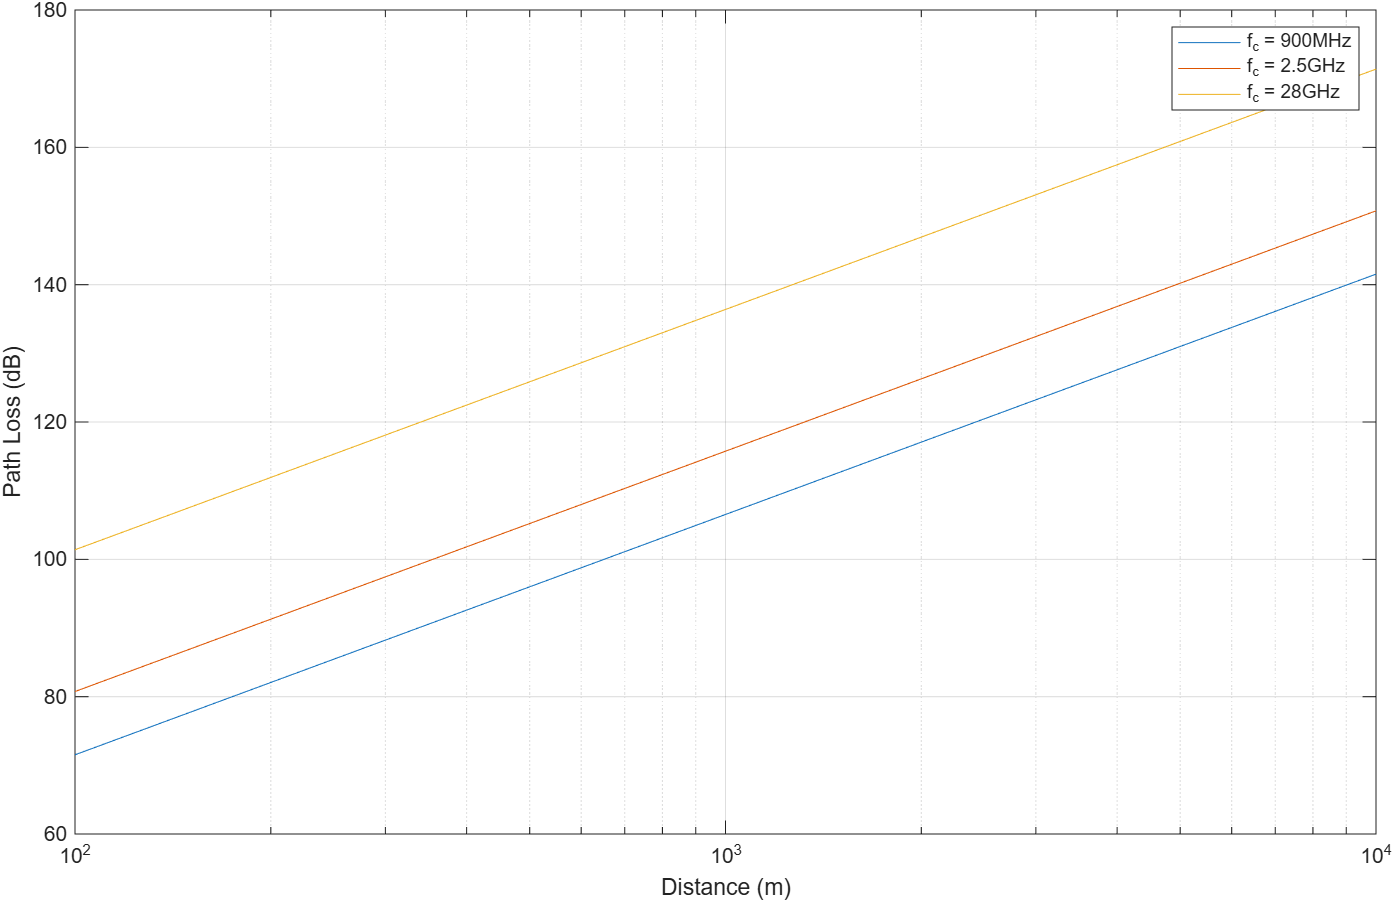
\includegraphics[width=\textwidth]{b_i.png}

\subsection{}
The three curves are all parallel to each other, shifted upwards as the frequency increases. They all maintain the same slope, since the slope factor $10 n \log_{10}(d/d_0)$ only depends on $n$ and $d$, which are the same across all the frequencies. Only the y intercept changes, which depends on $f_c$.

In order to calculate the path loss in dB, we derive the following from Equation (1), where $d$ is in meters, $f_c$ is in Hz, and $c$ is the speed of light in meters per second, $3\cdot 10^8$:

\begin{align*}
	PL_{fs} &= \left( \frac{4 \pi d \cdot f_c}{c} \right)^2\\
	PL_{fs|dB} &= 20 \cdot \log_{10}(d) + 20 \cdot \log_{10}(f_c) + 20 \log_{10}(\frac{4\pi}{c})\\
	PL_{fs|dB} &= 20 \cdot \log_{10}(d) + 20 \cdot \log_{10}(f_c) - 147.56
\end{align*}

The initial path losses in linear units, $PL_{fs}$ are as follows:\\
$900$MHz: $20 \cdot \log_{10}(100) + 20 \cdot \log_{10}(900 \cdot 10^{6}) - 147.56 = 71.53$dB\\
$2.6$GHz: $20 \cdot \log_{10}(100) + 20 \cdot \log_{10}(2.6 \cdot 10^{9}) - 147.56 = 80.75$dB\\
$28$GHz: $20 \cdot \log_{10}(100) + 20 \cdot \log_{10}(28 \cdot 10^{9}) - 147.56 = 101.39$dB\\\\

From these we know that the difference between the $900$MHz and $2.6$GHz path loss is $9.22$dB, and between $900$MHz and $28$GHz is $29.86$, which matches the figure.

\subsection{}
The Fraunhofer distance can be found using the following equation: $d_R = 2L_a^2/\lambda$. We know that $L_a = 0.5$m, and wavelength $\lambda$ can be found with $\lambda = c/f$.\\\\

$900$MHz: $\frac{2 \cdot 0.5^2}{c/900 \cdot 10^{6}} = 1.5$m\\
$2.6$GHz: $\frac{2 \cdot 0.5^2}{c/2.6 \cdot 10^{9}} = 4.33$m\\
$28$GHz: $\frac{2 \cdot 0.5^2}{c/28 \cdot 10^{9}} = 46.67$m\\\\

All three frequencies have a Fraunhofer distance less than $100$m, implying that this is a reasonable reference distance for free space path loss.

\subsection{}
This is a modeling artifact as it was based on a mathematical model, rather than on a particular physical measurement taken at a particular time, which would take into account \textit{all} of the phenomena that affect loss. For example, this does not take into account the inability to penetrate buildings that starts around 28GHz. At these frequencies rain and humidity also begin to be a factor in in path loss.

\section{Nominal link budget and maximum range.}
\subsection{}
$P_{r|dB} = P_{t|dB} - PL_{dB}$\\
If $P_{r|dB} \geq P_{dB}^{*}$, then $P_{t|dB} \geq P_{dB}^{*} + PL_{dB}$\\\\

Substituting in these initial equations and Equation (1), then rearranging:
\begin{align*}
	P_{t|dB} &\geq P_{db}^{*} + PL_{0|dB} + 10 n \log_{10} \left(\frac{R}{d_0} \right)\\
	P_{t|dB} - P_{db}^{*} - PL_{0|dB} &\geq 10 n \log_{10} \left(\frac{R}{d_0} \right)\\
	\frac{P_{t|dB} - P_{db}^{*} - PL_{0|dB}}{10n} &\geq \log_{10}(R) - \log_{10}(d_0)\\
	\frac{P_{t|dB} - P_{db}^{*} - PL_{0|dB}}{10n} + \log_{10}(d_0) &\geq \log_{10}(R)\\
	10^{\frac{P_{t|dB} - P_{db}^{*} - PL_{0|dB}}{10n} + \log_{10}(d_0)} &\geq R\\
	d_0 10^{\frac{P_{t|dB} - P_{db}^{*} - PL_{0|dB}}{10n}} &\geq R
\end{align*}

In order to plot, we find the value for path loss at the reference distance $PL_{0|dB}$:\\
\begin{align*}
	PL_{0|dB} &= 20 \cdot \log_{10}(d) + 20 \cdot \log_{10}(f_c) + 20 \log_{10}(\frac{4\pi}{c})\\
	PL_{0|dB}	&= 20 \cdot \log_{10}(100) + 20 \cdot \log_{10}(900 \cdot 10^{6}) + 20 \log_{10}(\frac{4\pi}{c})\\
	PL_{0|dB} &= 40 + 179.085 + (-147.56)\\
	PL_{0|dB} &= 71.53\text{dB}
\end{align*}

We also know that $P_{dB}^{*} = -100$dBm, $d_0=100$m, and $P_{t|dB} = 43$dBm, which allows us to further simplify the expression to:
\begin{align*}
	100 \cdot 10^{\frac{43 - (-100) - 71.53}{10n}} &\geq R\\
	100 \cdot 10^{\frac{71.47}{10n}} &\geq R
\end{align*}

This creates a plot as shown below. The Y axis is shown in kilometers, as the numbers in meters are too large to read easily.

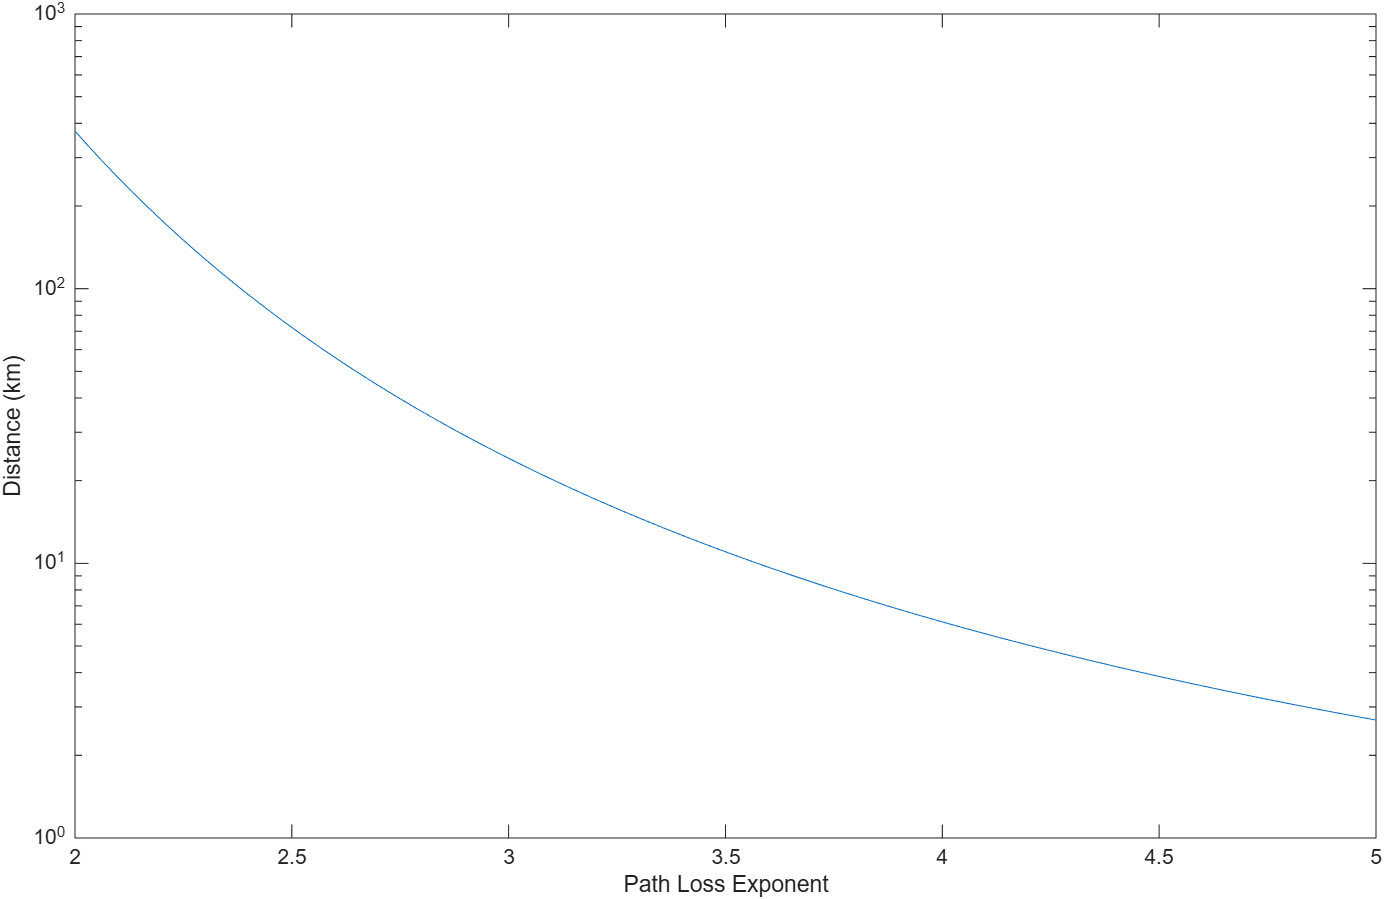
\includegraphics[width=\textwidth]{c_ii.png}

\subsection{}
\begin{center}
	\begin{tabular}{||c | c c c||} 
		\hline
		 $n$ & $2$ & $2.7$ & $3.5$ \\ [0.5ex] 
		\hline
		 R & $374.542$km & $44.365$km & $11.015$km \\ 
		\hline
	\end{tabular}
\end{center}

\subsection{}
The value of R at $n=2$ is unlikely to match reality, as it is many times the radius of the earth. As R increases, we are likely to find obstacles between transmitter and receiver. Even without buildings or other obstacles, the curvature of the earth will begin to interfere with the signal. If we consider a satellite or aerial system, we will get ionospheric and other atmospheric effects.

\subsection{}
As we add shadowing and fading margin, we need to increase the required transmit power $P_{t|dB}$, as shadowing increases losses.

\section{Estimate the model parameters.}
Let us first verify that the reference distances used satisfy $d_0 \geq d_R$:\\
Dataset A:\\
$\lambda = c/f = \frac{3\cdot 10 ^8}{900\cdot 10^6} = 0.33$m\\
$\frac{2(0.5)^2}{0.33} = 1.5$m\\\\
Dataset B:
$\lambda = c/f = \frac{3\cdot 10 ^8}{2.4\cdot 10^9} = 0.125$m\\
$\frac{2(0.05)^2}{0.125} = 0.04$m\\\\

This shows that both datasets are using correct reference distances.\\\\

Now let's compute $PL_{0|dB}$ for each dataset.\\
Dataset A:\\
\begin{align*}
	PL_{0A|dB} &= 20 \cdot \log_{10}(100) + 20 \cdot \log_{10}(900 \cdot 10^6) - 147.56\\
	PL_{0A|dB} &= 40 + 179.085 - 147.56 = 71.53\text{dB}
\end{align*}

Dataset B:\\
\begin{align*}
	PL_{0A|dB} &= 20 \cdot \log_{10}(1) + 20 \cdot \log_{10}(2.4 \cdot 10^9) - 147.56\\
	PL_{0A|dB} &= 0 + 187.604 - 147.56 = 40.04\text{dB}
\end{align*}

\subsection{}
In order to determine the value of $n$ that provides the lowest MMSE, we begin with defining:\\
$J = \sum_{i=0}^{N} (L_{i|meas} - L_{i|model})^2$

This decomposes to:

\begin{align*}
	J(n) &= \sum_{i=0}^{N} (L_{i|meas} - PL_0 - 10n\log_{10}(\frac{d_i}{d_0}))^2\\
	J(n) &= \sum_{i=0}^{N} (L_{i|meas} - PL_0) ^ 2 - 20(L_{i|meas} - PL_0)\log_{10}(\frac{d_i}{d_0}) + 100n^2\log_{10}^2(\frac{d_i}{d_0})
\end{align*}

Now to find $\frac{dJ}{dn}$ we take the derivative of $J(n)/N$:

\begin{align*}
	\frac{dJ}{dn} = 0 &= \frac{1}{N}\sum_{i=0}^{N} \frac{20\log_{10}(\frac{d_i}{d_0})(10n\log_{10}(\frac{d_i}{d_0})) - (L_{i|meas} - PL_0)\log_{10}(10)}{\log_{10}(10)}\\
	n &= \frac{1}{N} \frac{\sum_{i=0}^{N}(L_i - PL_0)\log(\frac{d_i}{d_0})}{\sum_{i=0}^{N}10\log^2(\frac{d_i}{d_0})}
\end{align*}

Running the sum provides the following estimates:\\
Dataset A: $n = 3.1445$ \\
Dataset B: $n = 2.8475$ \\

\subsection{}
Using the sample estimator in the problem, we obtain:\\
Dataset A: $\sigma = 6.5196$ \\
Dataset B: $\sigma = 8.8542$ \\

\subsection{}

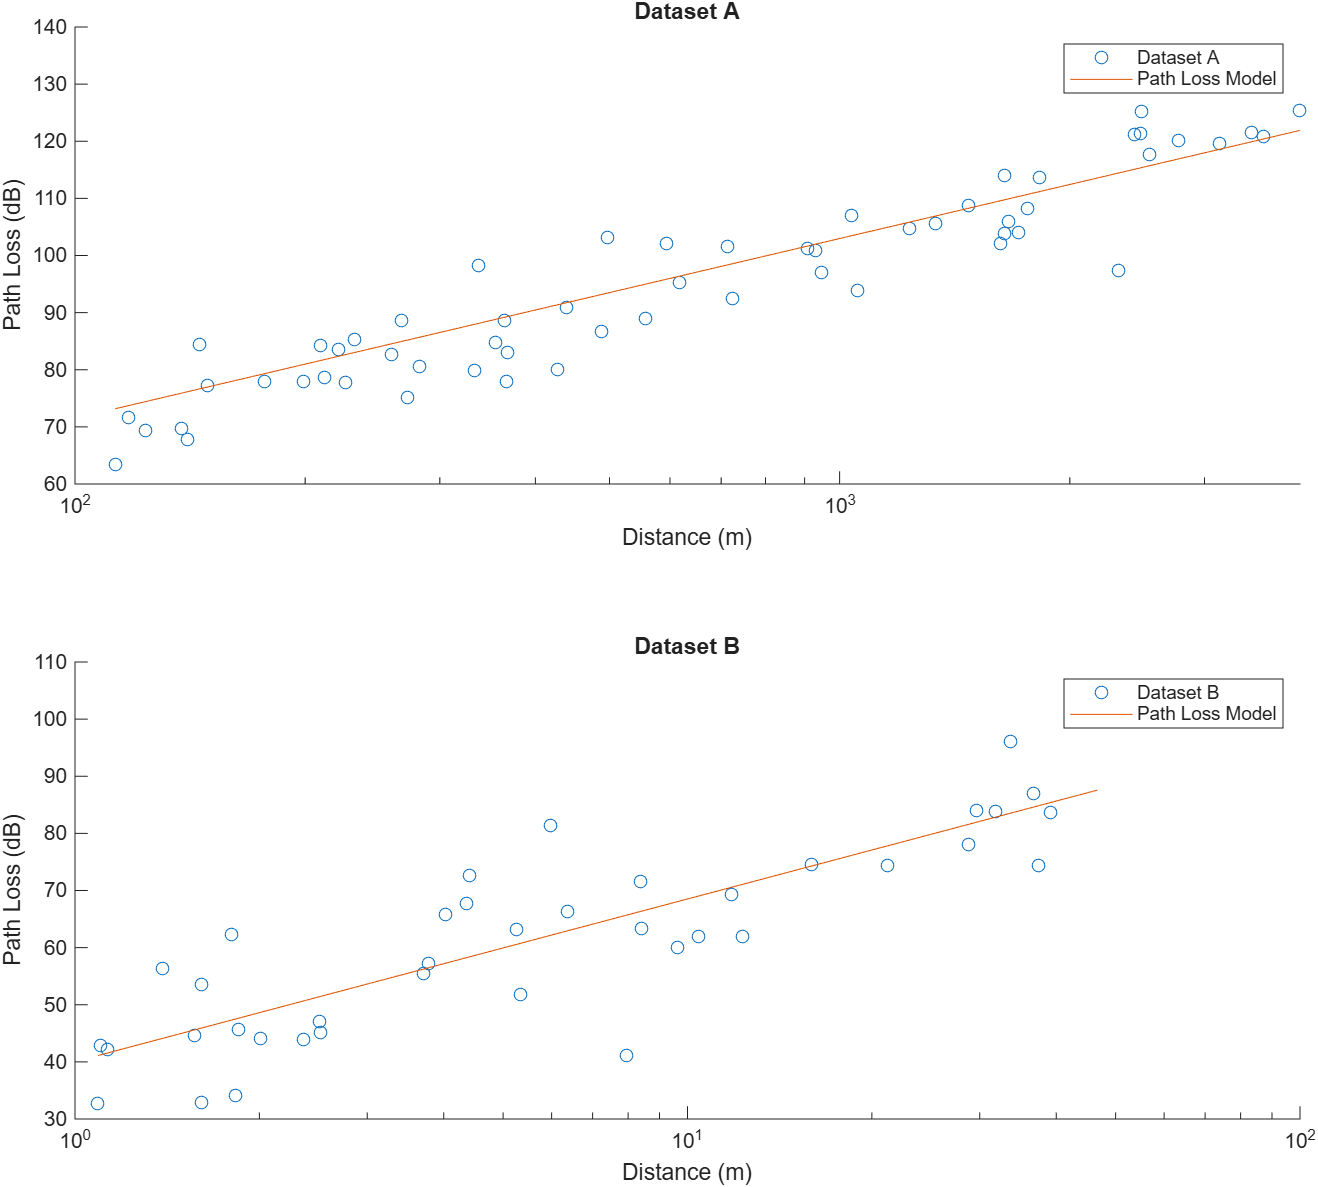
\includegraphics[width=\textwidth]{d_iii.png}\\

\subsection{}
Dataset A looks better on the figure than Dataset B, and has a smaller standard deviation, implying a better fit. There is more data for A ($M$), which will give a better fit. The higher $\sigma$ in B indicates that there is more variability in the environment (obstacles, buildings, other sources of multipath or attenuation), not that the model is necessarily worse.

\subsection{}
Urban area outdoor ($2.7-3.5$), from slide 18, module 2, fits A well.
The attenuation factor model in the lecture notes shows one measurement at $2.68$, but averages are higher, so B is low compared to the measurements from [Sei92b] (slide 43, module 2).

\section{Audit of a proposed solution.}
Line 33: Missing square term, should be: \verb|PL0A_dB = 20*log10(4*pi*d0A/lamA);|
Line 58: All following equations rely on \verb|f_cB| being expressed in Hz. Should be \verb|fcB = 2.4e9|.\\

Line 93: We expect that that linear unit cross check would match the logarithmic one, but it does not. This is expected, as the log scaling in dBs changes the residual calculations (squared error makes larger errors much more significant, especially as we are minimizing differences rather than ratios). This is especially significant if errors are not uniform across the plot. The only error here is to use the linear calculation as a cross check.\\

Line 131: Mixing linear and logarithmic units, should be:\\ 
\verb|L_check = PL0A_db + 10*nA_hat*log10(d_check/d0A);|

\subsection{}
Line 33 and 58, these caused the fit lines to very clearly not fit. 

\section{Verification Appendix}
\subsection{}
I did not use an AI tool for this assignment. 
\subsection{}
N/A
\subsection{}

\subsection{}
In problem d.i, I had not distributed the sum to both the numerator and denominator of the fraction, which caused issues in the computation of $n$. The results for $n$ were outside the normal range, which led me to recompute the equations.


\end{document}
